% Chapter 1

\chapter{Progettazione circuitale} % Write in your own chapter title
\label{Chapter3} 
\lhead{\emph{Progettazione circuitale}}

\section{Schema completo}
\begin{figure}[hbt!]
	\centering
	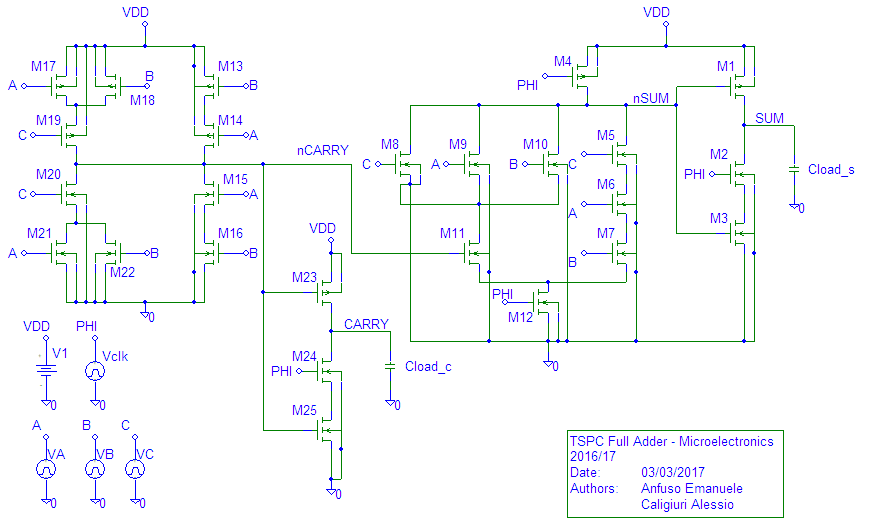
\includegraphics[width=1\textwidth]{figure/TSPC_FA_SchematicScreen.png}
	\caption{Schema completo del full-adder.}
	\label{fig:schemaCircuitale}
	\end{figure}
In fig. \ref{fig:schemaCircuitale} è mostrato lo schema completo del full-adder, così come simulato in \textit{SPICE}. Tutti i \textit{bulk} degli nMOS e dei pMOS sono stati collegati rispettivamente a massa e all'alimentazione positiva, in modo tale da assicurare la polarizzazione inversa delle giunzioni \textit{bulk - drain} e \textit{bulk - source} in ogni condizione operativa. Questa scelta è inoltre obbligata dalla realizzazione su silicio nella quale tutti i bulk degli nMOS (pMOS) corrispondono al medesimo substrato di tipo \textit{p} ("vasca" \textit{n-well}).

\section{Dimensionamento di massima}
\label{sec:sec_dimensionamentoMassima}
Il dimensionamento dei transistor prevede di iniziare dagli \textbf{stadi finali} \textit{2.2} e \textit{3} (in riferimento alla fig. \ref{fig:fig_schemaDaArticoloStadiCerchiati}), relativi rispettivamente ai MOS \textit{M1, M2, M3} e\textit{ M23, M24, M25} dello schema in fig. \ref{fig:schemaCircuitale}; entrambi hanno una capacità di carico $C_{load} = 100fF$, fornita dalle specifiche indicate in sezione \ref{sec:sec_fasiLavoro}.

Le capacità di gate di \textit{M1} e \textit{M3} costituiranno il carico dello stadio \textit{2.1} precedente; dipendendo queste dalle dimensioni dei MOS, si giustifica la necessità di iniziare dai finali e tornare indietro.
Si osservi che analogamente il carico dello stadio \textit{1} è dato dal parallelo delle capacità di gate di \textit{M23}, \textit{M25} (stadio \textit{2.2}) e \textit{M11} (stadio \textit{2.1}).

\subsection{Vincoli temporali e \textit{inverter equivalente}}
\label{subsec:specifiche}
Dalla frequenza operativa richiesta di $f_{clock} = 2GHz$ (ovvero periodo $T_{clock} = 500ps$) derivano vincoli temporali sulle fasi di valutazione e precarica, che devono andare a regime entro $T_{clock}/2 = 250ps$. Rispetto al formalismo usato in sezione \ref{sec:funzionamentoDinamicoCMOS}, questo vuol dire che i tempi di salita e di discesa dei singoli stadi devono restare entro tale limite: 
\begin{equation}
	\tau = \tau_{r} = \tau_{f} < T_{clock}/2 = 250ps
\end{equation}

A titolo precauzionale si fissa $\tau = 200ps$, tenendo conto anche dei $25ps$ dati come tempi di salita/discesa delle tensioni \textit{A, B, C, clock} in ingresso.

A questo punto si può applicare la formula \ref{eq:formulaRapportoAspetto}, impiegando i valori di $\mu _n$, $\mu _p$ e $C'_{ox}$ trovati in sezione \ref{sec:sec_mos}, ottenendo così i \textbf{rapporti d'aspetto dei MOS di un \textit{inverter equivalente}} che deve pilotare la data capacità di carico completando la carica entro il tempo definito. Si ricorda nuovamente che il risultato fornito da questa formula è decisamente più piccolo del necessario, a causa di approssimazioni ottimistiche sia sul tempo di carica/scarica (assunta lineare per facilità) sia sulla caratteristica del MOS, come già discusso.

\subsection{Dall'\textit{inverter equivalente} alle dimensioni dei MOS}
\label{subsec:daInverterAMOS}
Ai fini progettuali, ogni stadio del full-adder è assimilabile ad un \textit{inverter equivalente} dal momento che il segnale in uscita è \textit{alzato} a $V_{DD}$ da una serie/parallelo di pMOS ed \textit{abbassato} a massa da una serie/parallelo di nMOS; per ragioni geometriche entrambe queste combinazioni di transistor possono essere ricondotte ad un singolo componente di dimensioni opportune, considerando il caso peggiore.

Consideriamo per esempio la parte superiore dello stadio \textit{1}. Il percorso di corrente più sfavorevole si ha quando conducono solo \textit{M13} e \textit{M14} (o, analogamente, solo \textit{M17} e \textit{M19}). Due \textbf{MOS di uguale larghezza in serie} si possono valutare come un unico MOS con \textbf{rapporto d'aspetto equivalente} ridotto, come mostra la figura seguente.

\begin{figure}[hbt!]
	\centering
	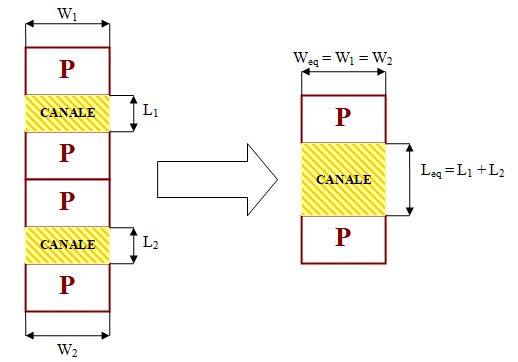
\includegraphics{figure/PMOS_series.png}
	\caption{Considerazioni geometriche sulle dimensioni di due pMOS in serie.}
	\label{fig:PMOS_series}
\end{figure}

Quando entrambi i transistor sono in conduzione, la corrente di drain percorre due canali, per una lunghezza totale $L_{eq} = L_1 + L_2$ e una larghezza costante $W_{eq} = W_1 = W_2 = W$. Se i due MOS hanno anche lunghezza di canale uguale ($L=L_1 = L_2$), il rapporto d'aspetto risulta dimezzato; infatti:
\begin{equation}
	\left ( \frac{W}{L} \right ) _{eq} = \frac{W}{L_1 + L_2} = \frac{W}{2 \cdot L} =  \frac{\left ( \frac{W}{L} \right ) _{1}}{2} = \frac{\left ( \frac{W}{L} \right ) _{2}}{2} 
\end{equation}
Questo vale sia per dispositivi a canale \textit{n} che a canale \textit{p}.
In generale, si può affermare che, con un numero $n \in  \mathbb{N}$ di MOS tutti uguali in serie, il rapporto d'aspetto del transistor equivalente è:
\begin{equation}
\left ( \frac{W}{L} \right ) _{eq} = \frac{\left ( \frac{W}{L} \right )}{n} 
\end{equation}
Una considerazione duale si può fare considerando il parallelo di MOS uguali, nel qual caso il rapporto d'aspetto del singolo è moltiplicato per il numero di dispositivi. Tuttavia questa considerazione non è d'interesse nella circostanza considerata, in quanto il caso peggiore in un parallelo si ha sempre quando conduce un solo MOS alla volta.

Per brevità non si riportano i conti sui singoli stadi, rimandando l'analisi degli stessi ai relativi script \textit{MATLAB}.

\subsection{Dimensioni geometriche dei MOS: risultati di \textit{MATLAB}}

Di seguito si riportano le dimensioni di massima dei MOS ottenute applicando le considerazioni precedenti; tali risultati sono stati calcolati con alcuni script \textit{MATLAB}.

\begin{table}[htb]
	\centering
	\begin{tabular}{c*{5}{c}}
		\toprule
		MOS & Canale & $W/L$ & W($\mu$m) & L($\mu$m) & Stadio\\
		\midrule
		M1 & p & 10 & 1.20 & 0.12 & Finale \textit{SUM} \\
		M2, M3 & n & 6 & 0.72 & 0.12 & " \\
		M4 & p & 2 & 0.24 & 0.12 & Generazione \textit{!SUM} \\
		M5, M6, M7 & n & 2 & 0.24 & 0.12 & " \\
		M8, M9, M10 & n & 2 & 0.24 & 0.12 & " \\
		M11 & n & 2 & 0.24 & 0.12 & " \\
		M12 & n & 2 & 0.24 & 0.12 & " \\
		M13, M14 & p & 6 & 0.72 & 0.12 & Generazione \textit{!CARRY} \\
		M15, M16 & n & 2 & 0.24 & 0.12 & " \\
		M17, M18, M19 & p & 6 & 0.72 & 0.12 & " \\
		M20, M21, M22 & n & 2 & 0.24 & 0.12 & " \\
		M23 & p & 8 & 0.96 & 0.12 & Finale \textit{CARRY} \\
		M24, M25 & n & 5 & 0.60 & 0.12 & " \\
		\bottomrule
	\end{tabular}
	\caption{Tabella delle dimensioni calcolate dei MOS, non valide.}
	\label{tab:dimensioniMosTeoriche}
\end{table}

\subsection{Prima simulazione \textit{pre-layout}}
La prima simulazione \textit{SPICE} (fig. \ref{fig:primaSimulazionePreLayout}) del circuito dimensionato come da tabella \ref{tab:dimensioniMosTeoriche} ha restituito dei risultati imbarazzanti: i segnali in uscita \textit{SUM} (in blu) e \textit{CARRY} (in verde) spesso non riescono a raggiungere le tensioni di alimentazione, perché le commutazioni sono troppo lente.

\begin{figure}[hbt!]
	\centering
	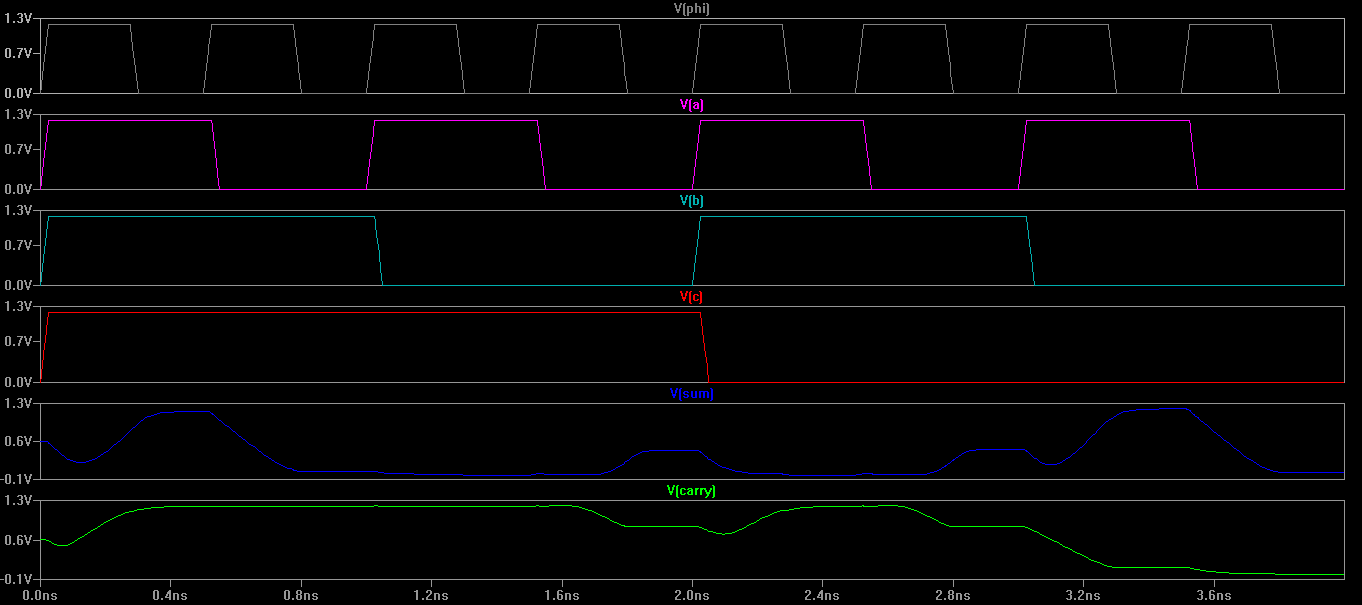
\includegraphics[width=1.3\textwidth, angle=90]{figure/sim_FA_Bad.png}
	\caption{Prima simulazione \textit{pre-layout} con dimensioni calcolate dei MOS.}
	\label{fig:primaSimulazionePreLayout}
\end{figure}

Per comprendere le cause di questo fallimento, abbiamo provato ad ingannare il simulatore semplificando il modello del MOS, esattamente come in sezione \ref{sec:ilModelloDiMicrowind}. Ne è risultata una simulazione, qui omessa, decisamente più aderente ai risultati attesi che ha testimoniato la bontà del dimensionamento effettuato ma chiaramente non attendibile dal momento che non ricalca il reale funzionamento dei MOS. Ad esempio, a causa del forte campo elettrico nella zona di canale dovuto alle ridotte dimensioni dei MOS (tutti a lunghezza minima), $\mu_n$ e $\mu_p$ non sono più costanti e diminuiscono rispetto ai valori calcolati, come già discusso in sezione \ref{sec:sec_caratteristicaMOS}.



\section{Fitting dei parametri: dimensioni definitive}
\label{sec:sec_fittingParametri}
Al fine di ottenere delle formule di progetto adeguate, sarebbe alquanto arduo utilizzare per i MOS il modello matematico \textit{SPICE level 3}. Abbiamo inizialmente provato a ricavare $\mu \cdot C'_{ox}$ e $V_{th}$ dalle curve caratteristiche \textit{level 3} di fig. \ref{fig:curveCaratteristicheReali} per utilizzare questi valori nella formula \ref{eq:formulaRapportoAspetto}, ottenendo dei transistor di larghezza assai elevata vista l'applicazione in questione.
Pertanto abbiamo scelto di cambiare approccio e operare in modo empirico: dopo un'attenta analisi dei segnali intermedi ottenuti mediante simulazioni, abbiamo agito sulle singole dimensioni dei transistor critici e, per approssimazioni successive, ci siamo avvicinati ad una soluzione soddisfacente sia dal punto di vista temporale che geometrico.

\MakeUppercase{è} stato necessario aumentare le dimensioni dei singoli transistor, in particolare di quelli finali che pilotano le uscite \textit{SUM} e \textit{CARRY} (stadi \textit{3} e \textit{2.2}). La tabella seguente riporta le nuove dimensioni.

\begin{table}[htb]
	\centering
	\begin{tabular}{c*{5}{c}}
		\toprule
		MOS & Canale & $W/L$ & W($\mu$m) & L($\mu$m) & Stadio\\
		\midrule
		M1 & p & 30 & 3.60 & 0.12 & Finale \textit{SUM} \\
		M2, M3 & n & 16 & 1.92 & 0.12 & " \\
		M4 & p & 10 & 1.20 & 0.12 & Generazione \textit{!SUM} \\
		M5, M6, M7 & n & 16 & 1.92 & 0.12 & " \\
		M8, M9, M10 & n & 10 & 1.20 & 0.12 & " \\
		M11 & n & 10 & 1.20 & 0.12 & " \\
		M12 & n & 16 & 1.92 & 0.12 & " \\
		M13, M14 & p & 24 & 2.88 & 0.12 & Generazione \textit{!CARRY} \\
		M15, M16 & n & 8 & 0.96 & 0.12 & " \\
		M17, M18, M19 & p & 24 & 2.88 & 0.12 & " \\
		M20, M21, M22 & n & 8 & 0.96 & 0.12 & " \\
		M23 & p & 30 & 3.60 & 0.12 & Finale \textit{CARRY} \\
		M24, M25 & n & 20 & 2.40 & 0.12 & " \\
		\bottomrule
	\end{tabular}
	\caption{Tabella delle dimensioni dei MOS dopo il \textit{fitting}.}
	\label{tab:dimensioniMosDefinitive}
\end{table}

\subsection{Simulazione \textit{pre-layout} soddisfacente}
La simulazione \textit{SPICE} \textit{pre-layout} finale mostra un corretto funzionamento del circuito. \MakeUppercase{è} agevole verificare che a fronte degli ingressi \textit{A}, \textit{B}, \textit{C}, le uscite \textit{SUM} e \textit{CARRY} forniscono i corretti valori logici e tensioni accettabili.

\begin{figure}[hbt!]
	\centering
	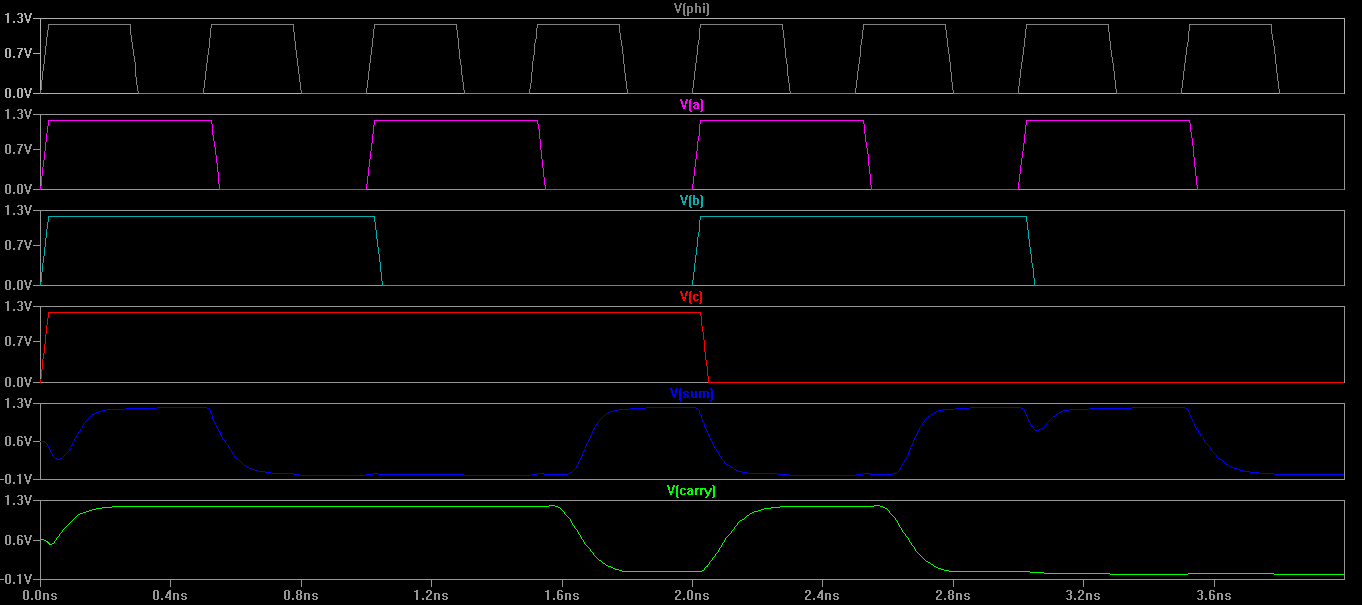
\includegraphics[width=1.5\textwidth, angle=90]{figure/sim_FA_Good.png}
	\caption{Simulazione \textit{pre-layout} soddisfacente.}
	\label{fig:simulazionePreLayoutSoddisfacente}
\end{figure}

Sarà necessario eseguire un'analoga simulazione \textit{post-layout}, ovvero dopo il disegno su silicio del circuito.